% !TeX root = ../analisi_2.tex

\section{Funzioni di più variabili}

\subsection{Funzioni di più variabili e grafici}

$f : A \subseteq \mathbb{R}^n \to \mathbb{R}$, $A \neq \emptyset$ e sia $A$ aperto \pencilnote{($f(x) = f(x_1, x_2, \dots, x_n)$)}.

\pencilnote{Come $f : [a, b] \to \mathbb{R}$, $y = f(x)$: il grafico ha una dim. in più.}

$n = 2$, $z = f(x, y)$

ovvero:
\[
f : A \subseteq \mathbb{R}^2 \to \mathbb{R}, \qquad z = f(x, y)
\]

\begin{center}
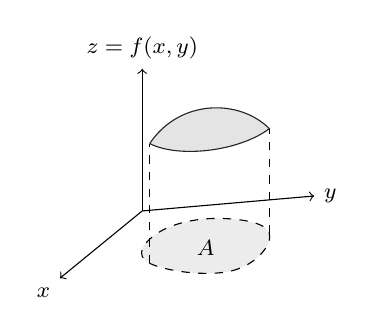
\begin{tikzpicture}[scale=0.95]
    % Assi 3D
    \draw[->] (0,0) -- (-1.1,-0.9) node[below left] {\footnotesize $x$};
    \draw[->] (0,0) -- (2.3,0.2) node[right] {\footnotesize $y$};
    \draw[->] (0,0) -- (0,1.9) node[above] {\footnotesize $z = f(x, y)$};

    % Regione A nel piano xy
    \draw[dashed, fill=gray!15] plot[smooth cycle, tension=0.75] coordinates {(0.1,-0.7) (1.2,-0.8) (1.7,-0.3) (1.0,-0.1) (0.2,-0.3)};
    \node at (0.85,-0.5) {\footnotesize $A$};

    % Superficie sopra A
    \draw[dashed] (0.1,-0.7) -- (0.1,0.9);
    \draw[dashed] (1.7,-0.3) -- (1.7,1.1);
    \draw[fill=gray!25, opacity=0.85] (0.1,0.9) .. controls (0.5,1.5) and (1.3,1.5) .. (1.7,1.1) .. controls (1.3,0.8) and (0.5,0.7) .. (0.1,0.9);
\end{tikzpicture}
\end{center}

\begin{example}
\begin{enumerate}
    \item $z = f(x, y) = x^2 + y^2$
    \begin{center}
    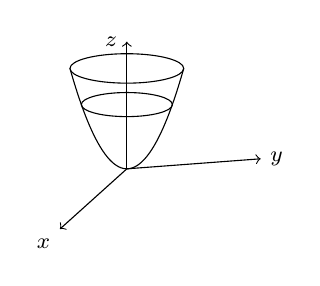
\begin{tikzpicture}[scale=0.85]
        \draw[->] (0,0) -- (-1.0,-0.9) node[below left] {\footnotesize $x$};
        \draw[->] (0,0) -- (2.0,0.15) node[right] {\footnotesize $y$};
        \draw[->] (0,0) -- (0,1.9) node[left] {\footnotesize $z$};
        % Paraboloide
        \draw[domain=-1:1, samples=50] plot ({0.85*\x}, {1.5*\x*\x});
        \draw (0,1.5) ellipse (0.85 and 0.22);
        \draw (0,0.96) ellipse (0.68 and 0.18);
    \end{tikzpicture}
    \end{center}

    \item $z = f(x, y) = \sqrt{x^2 + y^2}$
    \begin{center}
    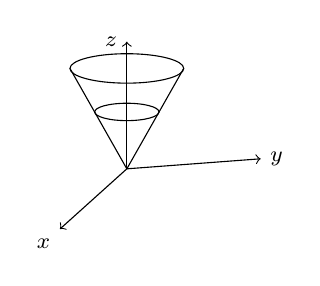
\begin{tikzpicture}[scale=0.85]
        \draw[->] (0,0) -- (-1.0,-0.9) node[below left] {\footnotesize $x$};
        \draw[->] (0,0) -- (2.0,0.15) node[right] {\footnotesize $y$};
        \draw[->] (0,0) -- (0,1.9) node[left] {\footnotesize $z$};
        % Cono
        \draw (0,0) -- (-0.85,1.5);
        \draw (0,0) -- (0.85,1.5);
        \draw (0,1.5) ellipse (0.85 and 0.22);
        \draw (0,0.85) ellipse (0.48 and 0.13);
    \end{tikzpicture}
    \end{center}
\end{enumerate}
\end{example}

\subsection{Limiti}

\begin{definition}
Sia $f : A \subseteq \mathbb{R}^2 \to \mathbb{R}$, $A \neq \emptyset$ e \underline{aperto}.

Sia $(x_0, y_0)$ un pto di acc. per $A$; diremo che $\lim_{(x, y) \to (x_0, y_0)} f(x, y) = l \in \mathbb{R}$ se
\[
\forall \varepsilon > 0 \ \exists I_\delta(x_0, y_0) : \vert f(x, y) - l \vert < \varepsilon \quad \forall (x, y) \in I_\delta(x_0, y_0) \cap A, \ (x_0, y_0) \neq (x, y)
\]
ovvero \pencilnote{($v = (x, y)$ e $v_0 = (x_0, y_0)$)}:
\[
\forall \varepsilon > 0 \ \exists \underbrace{I_\delta(v_0)}_{\text{usa nozione di distanza}} : \underbrace{\vert f(v) - l \vert}_{\text{val. assoluto}} < \varepsilon \quad \forall v \in I_\delta(v_0) \cap A, \ v \neq v_0
\]
Diremo che $\lim_{v \to v_0} f(x, y) = +\infty$ (o $-\infty$) se
\[
\forall M > 0 \ \exists I_\delta(v_0) : f(v) > M \ (\text{o } < -M) \quad \forall v \in I_\delta(v_0) \cap A \setminus \{v_0\}
\]
\end{definition}

\pencilnote{Valgono unicità, operazioni, T.P.S., etc.}

\begin{center}
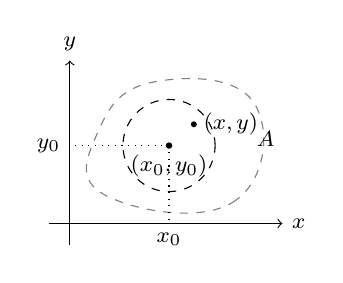
\begin{tikzpicture}[scale=0.9]
    \draw[->] (-0.3,0) -- (3.0,0) node[right] {\footnotesize $x$};
    \draw[->] (0,-0.3) -- (0,2.3) node[above] {\footnotesize $y$};
    \draw[dashed, gray] plot[smooth cycle, tension=0.8] coordinates {(0.5,0.4) (2.3,0.3) (2.6,1.7) (1.2,2.0) (0.4,1.3)};
    \node[right] at (2.5,1.2) {\footnotesize $A$};
    \fill (1.4,1.1) circle (1.3pt) node[below] {\footnotesize $(x_0, y_0)$};
    \draw[dashed] (1.4,1.1) circle (0.65);
    \fill (1.75,1.4) circle (1.2pt) node[right] {\footnotesize $(x, y)$};
    \draw[dotted] (1.4,1.1) -- (1.4,0) node[below] {\footnotesize $x_0$};
    \draw[dotted] (1.4,1.1) -- (0,1.1) node[left] {\footnotesize $y_0$};
\end{tikzpicture}
\end{center}

\underline{IDEA} per calcolo limite:
\[
\lim_{x \to x_0} \left( \lim_{y \to y_0} f(x, y) \right) \neq \lim_{y \to y_0} \left( \lim_{x \to x_0} f(x, y) \right) \quad \text{\pencilnote{(non sono necessariamente uguali)}}
\]

\pencilnote{(Non richiedo ``connessione'' perché considerando un intorno sono ``vicino'' $\implies$ è connesso)}

\begin{example}
\begin{enumerate}
    \item $f(x, y) = \begin{cases}
    1 & \text{se } \vert x \vert < \vert y \vert \\
    0 & \text{se } \vert x \vert > \vert y \vert
    \end{cases}$

    \pencilnote{$\vert x \vert < \vert y \vert \implies y < -\vert x \vert \lor y > \vert x \vert$}
    \begin{center}
    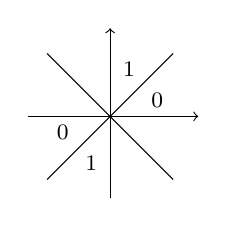
\begin{tikzpicture}[scale=0.8]
        \draw[->] (-1.3,0) -- (1.4,0);
        \draw[->] (0,-1.3) -- (0,1.4);
        \draw (-1.0,-1.0) -- (1.0,1.0);
        \draw (-1.0,1.0) -- (1.0,-1.0);
        \node at (0.3,0.75) {\footnotesize $1$};
        \node at (-0.3,-0.75) {\footnotesize $1$};
        \node at (0.75,0.25) {\footnotesize $0$};
        \node at (-0.75,-0.25) {\footnotesize $0$};
    \end{tikzpicture}
    \end{center}
    \[
    \lim_{(x, y) \to (0, 0)} f(x, y) = \nexists
    \]
    \[
    \lim_{x \to 0} \left( \lim_{y \to 0} f(x, y) \right) = \lim_{x \to 0} (f(x, 0)) = \lim_{x \to 0} 1 = 1
    \]
    \[
    \lim_{y \to 0} \left( \lim_{x \to 0} f(x, y) \right) = \lim_{y \to 0} (f(0, y)) = \lim_{y \to 0} 0 = 0
    \]
    sono diversi.

    \item $f(x, y) = x \sin\frac{1}{y} + y \sin\frac{1}{x}$

    \pencilnote{$\lim_{(x, y) \to (0, 0)} f(x, y) = 0$ perché? $\left( f(x, y) = \underbrace{x \sin\frac{1}{y}}_{\text{limitata } \cdot \text{ infinitesima } \to 0} + y \sin\frac{1}{x} \right)$
    \[
    \left\vert x \sin\frac{1}{y} + y \sin\frac{1}{x} \right\vert \le \vert x \vert + \vert y \vert < \sqrt{x^2 + y^2} + \sqrt{x^2 + y^2} = 2\underbrace{\sqrt{x^2 + y^2}}_{\delta} < \varepsilon
    \]
    (maggioro i seni con $1$ e poi dis. tri.) $\implies \delta < \frac{\varepsilon}{2} \implies$ il lim. esiste.

    Ma non posso fare il limite prima per $x$ e poi per $y$ (o viceversa) poiché $\lim_{x \to 0} \left( \underbrace{\lim_{y \to 0} x \sin\frac{1}{y}}_{\nexists} \right) = \nexists$.}

    \item $\lim_{(x, y) \to (0, 0)} \frac{x^2 - y^2}{x^2 + y^2} = \nexists$ \quad \pencilnote{(verrebbe $1$ e $-1$)}

    \item $\lim_{(x, y) \to (0, 0)} \frac{xy}{x^2 + y^2} = ?$ Se esiste deve essere $0$.

    Calcolo lungo la bisettrice ($y = x$): $\lim_{x \to 0} f(x, x) = \frac{x^2}{2x^2} = \frac{1}{2}$.

    Dunque il limite non esiste.

    \item \pencilnote{$\lim_{(x, y) \to (0, 0)} \frac{x y^2}{x^2 + y^4} = \nexists$

    Considero una qualunque retta: $\lim_{x \to 0} f(x, mx) = \lim_{x \to 0} \frac{m^2 x^3}{x^2 + m^4 x^4} = \lim_{x \to 0} \frac{m^2 x}{1 + m^4 x^2} = 0 \quad \forall m$ (ma non basta usare le rette).

    Uso le parabole:
    \begin{itemize}
        \item $\lim_{x \to 0} f(x, mx^2) = \lim_{x \to 0} \frac{m^2 x^5}{x^2 + m^4 x^8} = 0 \quad \forall m$
        \item $\lim_{y \to 0} f(my^2, y) = \lim_{y \to 0} \frac{m y^4}{m^2 y^4 + y^4} = \lim_{y \to 0} \frac{m}{m^2 + 1} = \nexists$ (dipende da $m$)
    \end{itemize}
    $\triangle$ Guarda ordine di infinitesimo.}
\end{enumerate}
\end{example}

\begin{oss}
Se $\lim_{(x, y) \to (x_0, y_0)} f(x, y) = l \implies \forall \varphi(t) = (x(t), y(t))$ tale che $\varphi(t_0) = (x_0, y_0)$ deve risultare che
\[
\lim_{t \to t_0} f(\varphi(t)) = \lim_{t \to t_0} f(x(t), y(t)) = l \quad \text{se il limite } \exists
\]
\end{oss}

\subsection{Continuità}

\begin{definition}
Sia $f : A \subseteq \mathbb{R}^2 \to \mathbb{R}$, $A \neq \emptyset$ e aperto.

Sia $(x_0, y_0) \in A$. $f$ si dice \underline{continua} in $(x_0, y_0)$ se
\[
\lim_{(x, y) \to (x_0, y_0)} f(x, y) = f(x_0, y_0) \iff \forall \varepsilon > 0 \ \exists \delta > 0 : \vert f(x, y) - f(x_0, y_0) \vert < \varepsilon \quad \forall (x, y) \in I_\delta(x_0, y_0) \cap A
\]
\end{definition}

\pencilnote{Insiemi particolari se $f$ è continua ($c \in \mathbb{R}$):
\begin{itemize}
    \item $\{ f(x, y) > c \}$ (o $< c$) aperti (sopralivelli o sottolivelli)
    \item $\{ f(x, y) \ge c \}$ (o $\le c$) chiusi
    \item $\{ (x, y) : f(x, y) = c \}$ curve di livello
\end{itemize}}

\begin{center}
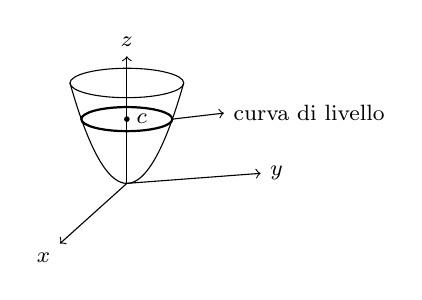
\begin{tikzpicture}[scale=0.85]
    \draw[->] (0,0) -- (-1.0,-0.9) node[below left] {\footnotesize $x$};
    \draw[->] (0,0) -- (2.0,0.15) node[right] {\footnotesize $y$};
    \draw[->] (0,0) -- (0,1.9) node[above] {\footnotesize $z$};
    % Paraboloide con curva di livello z = c
    \draw[domain=-1:1, samples=50] plot ({0.85*\x}, {1.5*\x*\x});
    \draw (0,1.5) ellipse (0.85 and 0.22);
    \draw[thick] (0,0.96) ellipse (0.68 and 0.18);
    \fill (0,0.96) circle (1.2pt) node[right] {\footnotesize $c$};
    \draw[->] (0.68,0.96) -- (1.45,1.05) node[right] {\footnotesize \pencilnote{curva di livello}};
\end{tikzpicture}
\end{center}
